\section{Overdraft events (exploratory)}
\label{sec:overdraft}

An overdraft warning needs a different quantity from any interval: the
probability that the booked end-of-day balance is below a threshold $u$ on
at least one of days $1, \dots, h$ after the origin (the origin day itself
is not counted). We scored that event at two thresholds:
\begin{itemize}
\item $u = 0$: a \emph{negative booked end-of-day balance}. Whether the
  bank treated it as an overdraft, or charged for it, is not in the data;
\item $u$ = the account's own tenth percentile of daily balances over the
  past year, a dip that is common enough to measure well.
\end{itemize}
\textbf{The forecasts:}
\begin{itemize}
\item \textbf{V2:} the share of its Monte Carlo paths whose running
  minimum falls below $u$, from the frozen configuration and seed;
\item \textbf{CP-noKF:} the same, from its paths;
\item \textbf{B-EQp:} the account's past $h$-day balance \emph{paths},
  shifted to today's balance;
\item \textbf{B-SRp:} the schedule plus past residual paths;
\item \textbf{the account's climatology (CLIM):} the share of its past
  $h$-day windows in which its own balance fell below $u$.
\end{itemize}
All empirical forecasts are coherent path forecasts over the same
\R{c/lookback} days. Table~\ref{tab:overdraft} gives the prevalence and
Brier scores, on held-out accounts (with development in brackets);
Figure~\ref{fig:overdraft} shows the reliability.

\begin{table}[t]
\centering\scriptsize\setlength{\tabcolsep}{3.5pt}
\begin{tabular}{ll r rrrrr}
\toprule
Event & $h$ & prevalence (\%) & V2 & CP-noKF & B-EQp & B-SRp & CLIM\\
\midrule
below 0 & \hA & \R{xh/s5/u0/7/prevalence} {\scriptsize(\R{xd/s5/u0/7/prevalence})} & \R{xh/s5/u0/7/brier_V2} & \R{xh/s5/u0/7/brier_CP-noKF} & \R{xh/s5/u0/7/brier_B-EQp} & \R{xh/s5/u0/7/brier_B-SRp} & \R{xh/s5/u0/7/brier_CLIM}\\
 & \hB & \R{xh/s5/u0/30/prevalence} {\scriptsize(\R{xd/s5/u0/30/prevalence})} & \R{xh/s5/u0/30/brier_V2} & \R{xh/s5/u0/30/brier_CP-noKF} & \R{xh/s5/u0/30/brier_B-EQp} & \R{xh/s5/u0/30/brier_B-SRp} & \R{xh/s5/u0/30/brier_CLIM}\\
 & \hC & \R{xh/s5/u0/90/prevalence} {\scriptsize(\R{xd/s5/u0/90/prevalence})} & \R{xh/s5/u0/90/brier_V2} & \R{xh/s5/u0/90/brier_CP-noKF} & \R{xh/s5/u0/90/brier_B-EQp} & \R{xh/s5/u0/90/brier_B-SRp} & \R{xh/s5/u0/90/brier_CLIM}\\
\addlinespace
below own tenth pct. & \hA & \R{xh/s5/u10/7/prevalence} {\scriptsize(\R{xd/s5/u10/7/prevalence})} & \R{xh/s5/u10/7/brier_V2} & \R{xh/s5/u10/7/brier_CP-noKF} & \R{xh/s5/u10/7/brier_B-EQp} & \R{xh/s5/u10/7/brier_B-SRp} & \R{xh/s5/u10/7/brier_CLIM}\\
 & \hB & \R{xh/s5/u10/30/prevalence} {\scriptsize(\R{xd/s5/u10/30/prevalence})} & \R{xh/s5/u10/30/brier_V2} & \R{xh/s5/u10/30/brier_CP-noKF} & \R{xh/s5/u10/30/brier_B-EQp} & \R{xh/s5/u10/30/brier_B-SRp} & \R{xh/s5/u10/30/brier_CLIM}\\
 & \hC & \R{xh/s5/u10/90/prevalence} {\scriptsize(\R{xd/s5/u10/90/prevalence})} & \R{xh/s5/u10/90/brier_V2} & \R{xh/s5/u10/90/brier_CP-noKF} & \R{xh/s5/u10/90/brier_B-EQp} & \R{xh/s5/u10/90/brier_B-SRp} & \R{xh/s5/u10/90/brier_CLIM}\\
\bottomrule
\end{tabular}
\caption{Overdraft events on held-out Berka (exploratory): prevalence (\%,
pooled over origins; development in brackets) and Brier scores (mean over
origins; lower is better). \R{xh/s5/u0/30/forecasts} origins per horizon in
\R{xh/s5/u0/30/accounts} accounts. Account-equal Brier scores, Brier skill
against CLIM with \R{c/ci-level}\% account-bootstrap intervals, and the
development results are in
\texttt{paper/results/exploratory*/s5-overdraft/}.}
\label{tab:overdraft}
\end{table}

\paragraph{Below zero: at a month or more, no method beats the account's
climatology.} The event is rare: \R{xh/s5/u0/7/prevalence},
\R{xh/s5/u0/30/prevalence} and \R{xh/s5/u0/90/prevalence}\% of origins at
\hA, \hB\ and \hC\ days on held-out accounts.
\begin{itemize}
\item \textbf{At \hB\ and \hC\ days,} each of the four model-based
  forecasts has a higher Brier
  score than CLIM. V2's Brier skill against CLIM is \R{xh/s5/u0/30/bss_V2}
  and \R{xh/s5/u0/90/bss_V2}.
\item \textbf{At \hA\ days,} only B-EQp beats CLIM: skill
  \R{xh/s5/u0/7/bss_B-EQp} [\R{xh/s5/u0/7/bss_B-EQp_lo},
  \R{xh/s5/u0/7/bss_B-EQp_hi}], and \R{xd/s5/u0/7/bss_B-EQp} on development.
  The held-out prevalence of this cell is below the \R{c/prev-min}\% our
  specification set for reliable results, so we mark it unreliable.
\end{itemize}

\paragraph{Below the account's own tenth percentile: every method beats
climatology.} At \hB\ days the Brier skills against CLIM are:
\begin{itemize}
\item V2: \R{xh/s5/u10/30/bss_V2} [\R{xh/s5/u10/30/bss_V2_lo},
  \R{xh/s5/u10/30/bss_V2_hi}];
\item B-EQp: \R{xh/s5/u10/30/bss_B-EQp}.
\end{itemize}
The schedule-based forecasts are best at \hA\ days and B-EQp at \hB\ and \hC\ days,
mirroring the horizon reversal in CRPS.

\begin{table}[t]
\centering\scriptsize\setlength{\tabcolsep}{3.5pt}
\begin{tabular}{ll r rrrrr}
\toprule
Event & $h$ & observed (\%) & V2 & CP-noKF & B-EQp & B-SRp & CLIM\\
\midrule
below 0 & \hA & \R{xh/s5c/u0/7/V2/observed} & \R{xh/s5c/u0/7/V2/diff} & \R{xh/s5c/u0/7/cp-nokf/diff} & \R{xh/s5c/u0/7/B-EQp/diff} & \R{xh/s5c/u0/7/B-SRp/diff} & \R{xh/s5c/u0/7/clim/diff}\\
 & \hB & \R{xh/s5c/u0/30/V2/observed} & \R{xh/s5c/u0/30/V2/diff} & \R{xh/s5c/u0/30/cp-nokf/diff} & \R{xh/s5c/u0/30/B-EQp/diff} & \R{xh/s5c/u0/30/B-SRp/diff} & \R{xh/s5c/u0/30/clim/diff}\\
 & \hC & \R{xh/s5c/u0/90/V2/observed} & \R{xh/s5c/u0/90/V2/diff} & \R{xh/s5c/u0/90/cp-nokf/diff} & \R{xh/s5c/u0/90/B-EQp/diff} & \R{xh/s5c/u0/90/B-SRp/diff} & \R{xh/s5c/u0/90/clim/diff}\\
\addlinespace
below own tenth pct. & \hA & \R{xh/s5c/u10/7/V2/observed} & \R{xh/s5c/u10/7/V2/diff} & \R{xh/s5c/u10/7/cp-nokf/diff} & \R{xh/s5c/u10/7/B-EQp/diff} & \R{xh/s5c/u10/7/B-SRp/diff} & \R{xh/s5c/u10/7/clim/diff}\\
 & \hB & \R{xh/s5c/u10/30/V2/observed} & \R{xh/s5c/u10/30/V2/diff} & \R{xh/s5c/u10/30/cp-nokf/diff} & \R{xh/s5c/u10/30/B-EQp/diff} & \R{xh/s5c/u10/30/B-SRp/diff} & \R{xh/s5c/u10/30/clim/diff}\\
 & \hC & \R{xh/s5c/u10/90/V2/observed} & \R{xh/s5c/u10/90/V2/diff} & \R{xh/s5c/u10/90/cp-nokf/diff} & \R{xh/s5c/u10/90/B-EQp/diff} & \R{xh/s5c/u10/90/B-SRp/diff} & \R{xh/s5c/u10/90/clim/diff}\\
\bottomrule
\end{tabular}
\caption{Calibration in the large of the overdraft-event probabilities on
held-out Berka (exploratory, computed after the held-out run from its
stored events): the mean forecast probability minus the observed event
frequency, in percentage points, both pooled over the
\R{xh/s5c/u0/30/V2/forecasts} origins per horizon in
\R{xh/s5c/u0/30/V2/accounts} accounts. Positive: the method over-predicts
the event. The \R{c/ci-level}\% account-bootstrap intervals and the
development results are in \texttt{paper/results/exploratory*/s5-overdraft/citl.csv}.}
\label{tab:citl}
\end{table}

\paragraph{Calibration in the large is poor for the four model-based
forecasts.} Averaged over origins, V2, CP-noKF, B-EQp and B-SRp each give
the event a higher probability than its observed frequency, at both
thresholds and every horizon, on both splits (Table~\ref{tab:citl}); every \R{c/ci-level}\%
account-bootstrap interval of the difference excludes zero.
\begin{itemize}
\item \textbf{Below zero at \hC\ days,} V2's mean probability is
  \R{xh/s5c/u0/90/V2/mean_p}\% against \R{xh/s5c/u0/90/V2/observed}\%
  observed [interval of the difference \R{xh/s5c/u0/90/V2/diff_lo},
  \R{xh/s5c/u0/90/V2/diff_hi} points]; on development,
  \R{xd/s5c/u0/90/V2/mean_p}\% against \R{xd/s5c/u0/90/V2/observed}\%.
  B-EQp over-predicts least: \R{xh/s5c/u0/90/B-EQp/mean_p}\%.
\item \textbf{Below the tenth percentile at \hB\ days,} V2 gives
  \R{xh/s5c/u10/30/V2/mean_p}\% against \R{xh/s5c/u10/30/V2/observed}\%.
\item \textbf{The reliability curves} (Figure~\ref{fig:overdraft}) show
  the same bin by bin: they lie mostly below the diagonal. The exception is
  the lowest-probability bins for the tenth-percentile event at \hC\ days,
  where events are slightly more frequent than forecast. That matches V2's
  few misses below its intervals (\S\ref{sec:calibration}).
\end{itemize}
CLIM, the account's own past frequency, slightly under-predicts a negative
balance (\R{xh/s5c/u0/90/clim/diff} points at \hC\ days).

\begin{figure}[t]
\centering
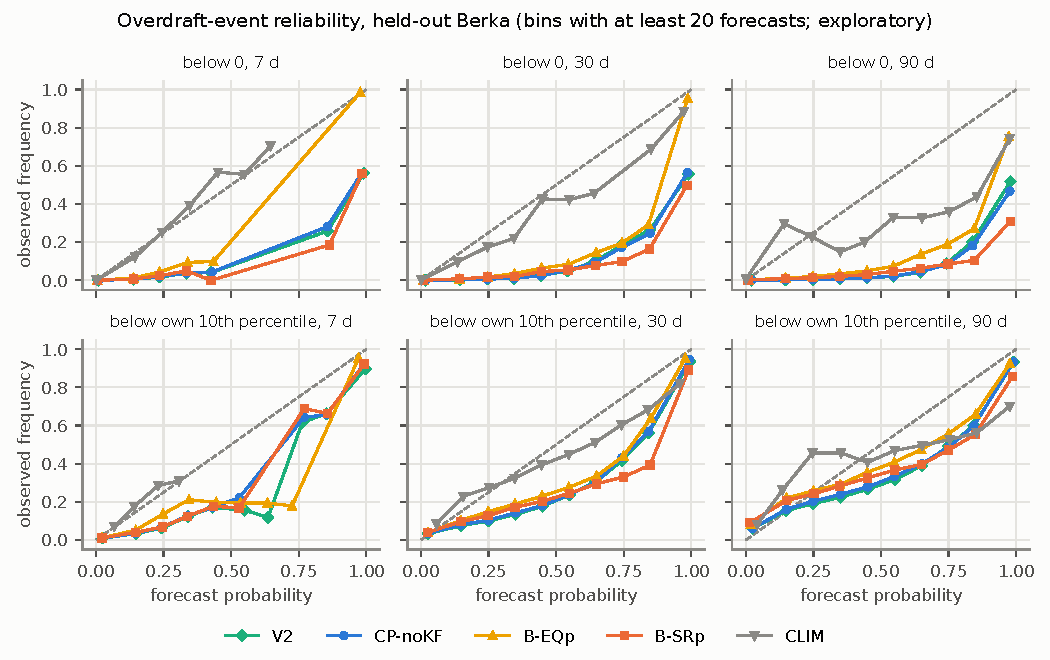
\includegraphics[width=\linewidth]{figures/overdraft-heldout.pdf}
\caption{Reliability of the overdraft-event probabilities on held-out Berka
(exploratory): observed frequency against forecast probability in ten
equal-width bins, shown where a bin holds at least twenty forecasts.
Below the diagonal: the method over-predicts the event. Bin counts are in
the exploratory held-out results.}
\label{fig:overdraft}
\end{figure}
